% This version of CVPR template is provided by Ming-Ming Cheng.
% Please leave an issue if you found a bug:
% https://github.com/MCG-NKU/CVPR_Template.

\documentclass[review]{cvpr}
%\documentclass[final]{cvpr}

\usepackage{times}
\usepackage{epsfig}
\usepackage{graphicx}
\usepackage{amsmath}
\usepackage{amssymb}
\usepackage{multirow}
\usepackage{caption}
\usepackage{subcaption}
\usepackage{array}

% Include other packages here, before hyperref.

% If you comment hyperref and then uncomment it, you should delete
% egpaper.aux before re-running latex.  (Or just hit 'q' on the first latex
% run, let it finish, and you should be clear).
\usepackage[pagebackref=true,breaklinks=true,colorlinks,bookmarks=false]{hyperref}

\newcommand{\lnote}[1]{\textcolor{blue}{\textbf{LR: #1}}}

\def\cvprPaperID{****} % *** Enter the CVPR Paper ID here
\def\confYear{CVPR 2021}
%\setcounter{page}{4321} % For final version only

% TODO dove pubblicare il codice:
% - https://github.com/rwightman/pytorch-image-models#models

\begin{document}

%%%%%%%%% TITLE
\title{\LaTeX\ Author Guidelines for CVPR Proceedings}

\author{First Author\\
Institution1\\
Institution1 address\\
{\tt\small firstauthor@i1.org}
% For a paper whose authors are all at the same institution,
% omit the following lines up until the closing ``}''.
% Additional authors and addresses can be added with ``\and'',
% just like the second author.
% To save space, use either the email address or home page, not both
\and
Second Author\\
Institution2\\
First line of institution2 address\\
{\tt\small secondauthor@i2.org}
}

\maketitle


%%%%%%%%% ABSTRACT
\begin{abstract}
Autonomous Vehicles (AVs) are almost certainly becoming a reality for the near future thanks to the substantial recent advances in computer vision.
To make this happen, it is of paramount importance to give to AVs the ability to understand the surrounding scene.
This paper presents a system capable to work in a real-time and online fashion, giving an immediate response to the arise of anomalies surrounding the AV, exploiting only the videos captured by a dash-mounted camera.
Our proposed architecture, called \emph{MOVAD}, is composed by two modules: a short-term memory to extract information related to the ongoing action, implemented by a Video Swin Transformer adapted to work in an online scenario, and a long-term memory module that considers remote past information thanks to the use of a Long-Short Term Memory (LSTM).
We evaluated the performance of our method on Detection of Traffic Anomaly (DoTA) dataset, a challenging collection of dash-mounted camera videos of accidents.
After an extensive ablation study, MOVAD is able to reach an AUC score of \anote{82.05\%}, surpassing the current state-of-the-art by $+2.75\%$ AUC.
Our code will be available on \url{https://github.com/IMPLabUniPr/movad}
\end{abstract}

%%%%%%%%% BODY TEXT
\section{Introduction}

%Intro
In order to make Autonomous Vehicles (AV) reliable in a real-world scenario, safety for every agent involved must be the focus of every self-driving system implementation.
This objective will be achieved once the AV has a clear understanding of the driving scene around it, focusing on the main visual cues that are needed for its correct behaviour, differentiating between normal and anomalous situations, so that it can react in real-time to make the safest decision.
It is necessary to track down all possible causes for the sake of accident avoidance, this must be done with both precision and promptness to assure the maximum reaction space.

%Task
Our work put the focus on video analysis captured by dash-mounted cameras, willing to improve the tools for driving scene interpretation in the context of Advanced Driver Assistance Systems (ADAS).
From this perspective, a driving scenario is quite hard to model since there are many information to take into account that can be exploited to define the driving scene.
There are plenty of possible accident classes that must be taken into account and to make matters worse, most of the times, it is quite hard to distinguish normal driving scenes from accident ones at frame level, which further enhances the problem's complexity.

%Anomaly
Though we know that accidents are a consequence of an anomalous driving scenario, it is non-trivial to define precise boundaries of what a driving anomaly is.
We can define an anomaly as an hazardous situation that can lead to an accident, but since the hazardousness prior to the accident may be determined subjectively by each individual, the time interval edges for an anomaly are not really clear and this is reflected in some dataset annotations.
Some attempts have been made to propose a deterministic method in the interest of defining an anomaly.
Yao et al. \cite{yao2019unsupervised} defines an anomaly as the window in which the accident happens, but since we want to prevent it, this might not be ideal in a prevention perspective.
Fang et al. \cite{fang2019dada} instead want to predict an accident willing to happen in the next 5 seconds labelling the anomaly start from the moment in which half part of the object involved in the accident appears in the view.
Yao et al. \cite{yao2020when} proposed a Detection of Traffic Anomaly (DoTA) dataset that takes into account When the anomalous event starts and ends, locates spatially Where all the involved agents are in each frame and What type of anomaly it is.
Their work formulates the anomaly start as the instant after which the accident is unavoidable.
As said before choosing that instant is quite subjective depending on the situation and personal biases, in fact Lung et al. \cite{lund2009riskperception} argues that risk perception is related to social constructs that reflect the cultural context in which people live in.

%TODO Saliency
%Determining an anomalous scene implies to evaluate the salient regions
Human's capability of evaluating danger on the fly is still a matter of study by neuroscientists.
When comparing machine to humans in the task of describing the content of an image we know that the latters perform better \cite{jiang2015salicon}.
Since we are aiming to develop a system capable of estimating danger in traffic video scenes it is worth emulating how humans focus on important regions or objects in images through saliency estimation.
The commonly adopted saliency definition is based on how pixels/regions stand out and is dependent of what kind of visual stimuli human respond to the most \cite{yan2013hierachical}.
Cornia et al.\cite{cornia2016saliency} proposed Multi-Level Network for Saliency Prediction (MLNET), an architecture for saliency estimation which simulates what human see at first glance, a step forward towards driving scene comprehension.

%TODO Breve accenno su tranformer
Transformer have become the most popular approach in computer vision tasks, dominating over CNN architectures, after the introduction of Vision Transformer (Dosovitskiy et al. \cite{DBLP:conf/iclr/DosovitskiyB0WZ21})  with which image patches are seen as tokens (word) in NLP applications, while keeping the architecture as similar as possible to the original.
A meaningful upgrade to this architecture, proposed by Liu et al. \cite{liu2021Swin}, was Swin Transformer.
Comparing to the previous architecture, the latter keeps a linear computational complexity to image size and builds hierarchical feature maps by using a shifting window mechanism on the window partition between consecutive self-attention layers, allowing for a significant enhance in modelling power while keeping efficiency in latency regards.
As a further proof, Video Swin Transfomer \cite{liu_video_2022} surpassed previous convolutional models for video recognition tasks by taking advantage of spatio-temporal locality of videos, that is, pixel that are closer to each other in spatio-temporal distance are more likely to be correlated.\\

%Contribution
Following the satisfying result of the previous works we propose to solve the problem of traffic anomaly detection in videos by using a Video Swin Transformer as our backbone network, adapting it to work in a real-time scenario, as expected from an ADAS implementation.
As a further contribution for our work we introduced a saliency map estimation model for each frame by using an MLNET, willing to let the model focus only on the most pertinent regions of the traffic scenes.
Finally we propose a relabelling of DoTA dataset adopting a different criterion of evaluation disentangled from the subjectivity and granting a deterministic method for estimating anomaly boundaries, allowing the largest possible reaction space while maintaining normal and anomalous scenes well separated.

In the next sections we will first introduce all the previous work at the state-of-the-art that led us into building the  architecture we are presenting, it will follow an overview of mathematical representation of our work and an in-depth explanation of all the components employed. 
Finally we will present our considerations and an ablation study where we will prove the superiority of our method compared to the state-of-the-art we are writing the article.
\section{Related}
\label{sec:related}

\noindent\textbf{Vision Transformers}
Transformers \cite{vaswani2017attention} are born as an architecture to solve sequence-to-sequence problems, handling long-range dependencies in a simple way with the advantage of a strong parallelization compared to state-of-the-art architectures such as RNN and derivatives.
Initially developed for text analysis tasks, transformers have also found application in the image field.
The seminal work \cite{DBLP:conf/iclr/DosovitskiyB0WZ21} first proposed a Vision Transformer (ViT), paving the way for a new generation of detectors, alternative to CNN.
Afterwards, with the aim of improving the performance in terms of accuracy of the results and decreasing the computational need, variants such as the Swin Tranformers \cite{liu2021Swin} were born.
In order to reduce the computational cost of the self-attention mechanism, authors proposed a shifted-windowing scheme to compute self-attention on smaller non-overlapping windows, introducing cross-window connection to cope with the lack of connections between different regions of the image.
As a direct evolution of Swin Tranformers, to process video instead of images, a new architecture was proposed in \cite{liu_video_2022}.
The authors proposed to approximate spatiotemporal self-attention by compute self-attention locally, extending spatial domain to the spatiotemporal domain.

\noindent\textbf{Traffic Anomaly Detection}
To detect anomaly in video, in \cite{hasan2016learning}, authors proposed a convolutional AutoEncoder (ConvAE) trained only on normal frames with the objective of frames reconstruction.
In \cite{luo2017remembering, wang2018abnormal}, authors used Convolutional LSTM Auto-Encoder as framework to encode appearance and motion.
Authors of AnoPred \cite{liu2018future} proposed a multi-task loss which include image intensity, optical flow, gradient, and adversarial losses for video frame-level anomaly detection which apply a UNet to predict a future RGB frame.
In \cite{yao2019unsupervised}, authors proposed an unsupervised method which tracks traffic participants trajectories and detect anomaly monitoring prediction consistency.
In TRN model \cite{xu2019temporal}, authors coupled the action detection task with the future action anticipation during the training.
To predict the action, they use both the historical temporal dependencies modeled by a RNN and the anticipation of the future via a temporal decoder.
In 2020, authors of \cite{9712446} proposed a new dataset of video anomaly detection called Detection of Traffic Anomaly (DoTA).
% TODO check paper https://paperswithcode.com/paper/an-attention-guided-multistream-feature

% Online Action Detection
% Temporal Recurrent Networks for Online Action Detection
% Long Short-Term Transformer for Online Action Detection

\section{Memory-augmented Online VAD}
\label{sec:theory}

\fboxsep=1mm%padding thickness
\fboxrule=1pt%border thickness

\begin{figure}[!t]
            \centerline{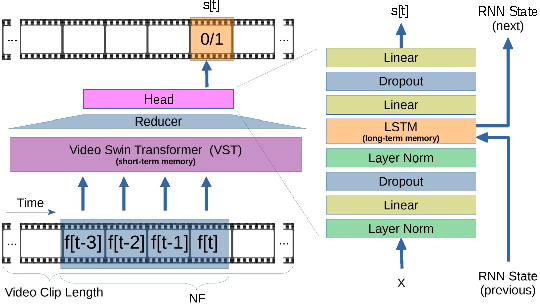
\includegraphics[clip, width=\linewidth]{images/arch-rx-cropped.pdf}}
        \caption{The online frame-level Video Anomaly Detection (VAD) architecture. $f[t]$ is the frame at time $t$, $x$ the output of the Reducer, $\mathit{NF}$ the number of frames in input to the VST, $s[t]$ the anomaly classification score of the frame $f[t]$.\label{fig:arch}}
\end{figure}

In this section the MOVAD architecture is described.  
The model is composed by: a short-term memory module and a classification Head that includes a long-term memory module (see Fig.~\ref{fig:arch}). 
Taking inspiration from~\cite{xu2021long}, recently observed frames have been taken into account as a source of information related to the ongoing action, and past frames to take into account the context.

\noindent\textbf{Short-term memory module.}
Since we are dealing with the online version of VAD task, the only information available to the system, at any given time, are the current and the past frames.
In order to implement this module, we selected the Video Swin Transformer (VST)~\cite{liu_video_2022} over ViViT~\cite{Arnab_2021_ICCV} due to its superior performance, and over an RNN given its ability to process frames in parallel.
Originally born to carry out the Video Action Classification task, analyzing all the frames in one step, we adapted to perform single-frame classification using few of them.
In particular, it considers only a small temporal window of $\mathit{NF}$ frames of the video, going from the current frame at time $t$ to the previous frames at time $t-\left(\mathit{NF}-1\right)$.
VST takes as input a video with size $\mathit{NF} \times H \times W \times 3$, where $\mathit{NF = 4}$, $H$ e $W$ correspond to the number of frames, height, width and RGB channels, respectively.
The model internally splits the frames in non-overlapping 3D patches, partitioning the video in $\frac{\mathit{NF}}{2} \times \frac{H}{4} \times \frac{W}{4}$ 3D tokens, projecting the features to an arbitrary dimension $C$.
The rest of the architecture is similar to the original Swin Transformer~\cite{liu2021Swin}, with four stages of Video Swin Transformer blocks, interspersed with $2\times$ spatial down-sampling in the patch merging layer.

\noindent\textbf{Long-term memory module.}
The output of VST goes through Adaptive Average Pool 3D layer (Reducer in Fig.~\ref{fig:arch}) and, finally, enter inside the classification Head.
As shown in Fig.~\ref{fig:arch}, the Head is composed by a series of normalization layers, linear layers and dropout, alternating. 
It deals with long-term memory thanks to a LSTM module inserted after the last normalization layer.
This module is composed by three cells stacked together to form a stacked LSTM.
The state, composed by an hidden state $h[t]$ and cell state $c[t]$, is updated whenever a new frame is available.
The LSTM receives in input a features block of $[B, 1024]$, where $B$ is the batch size, and returns a block of same size together with the state of the cells.
Because the state is relatively small, the module is very efficient and leads to a fixed and limited additional computational cost.
For each frame $f[t]$, the model outputs the anomaly classification score $s[t] \in [0,1]$, where $0$ means no anomaly and $1$ means the frame is anomalous.
A weighted cross-entropy loss was chosen to train the model, giving higher weight to the anomaly class, in order to reflect the distribution of the data.

% copyright image frame: <a href="https://www.freepik.com/free-vector/realistic-vector-icon-film-tape-strip-with-white-square-isolated-white-cinema-concept_31096470.htm#query=video%20frame&position=31&from_view=keyword">Image by user15245033</a> on Freepik
\section{Experiments}
\label{sec:experiments}

\begin{figure}[t]
\centering
	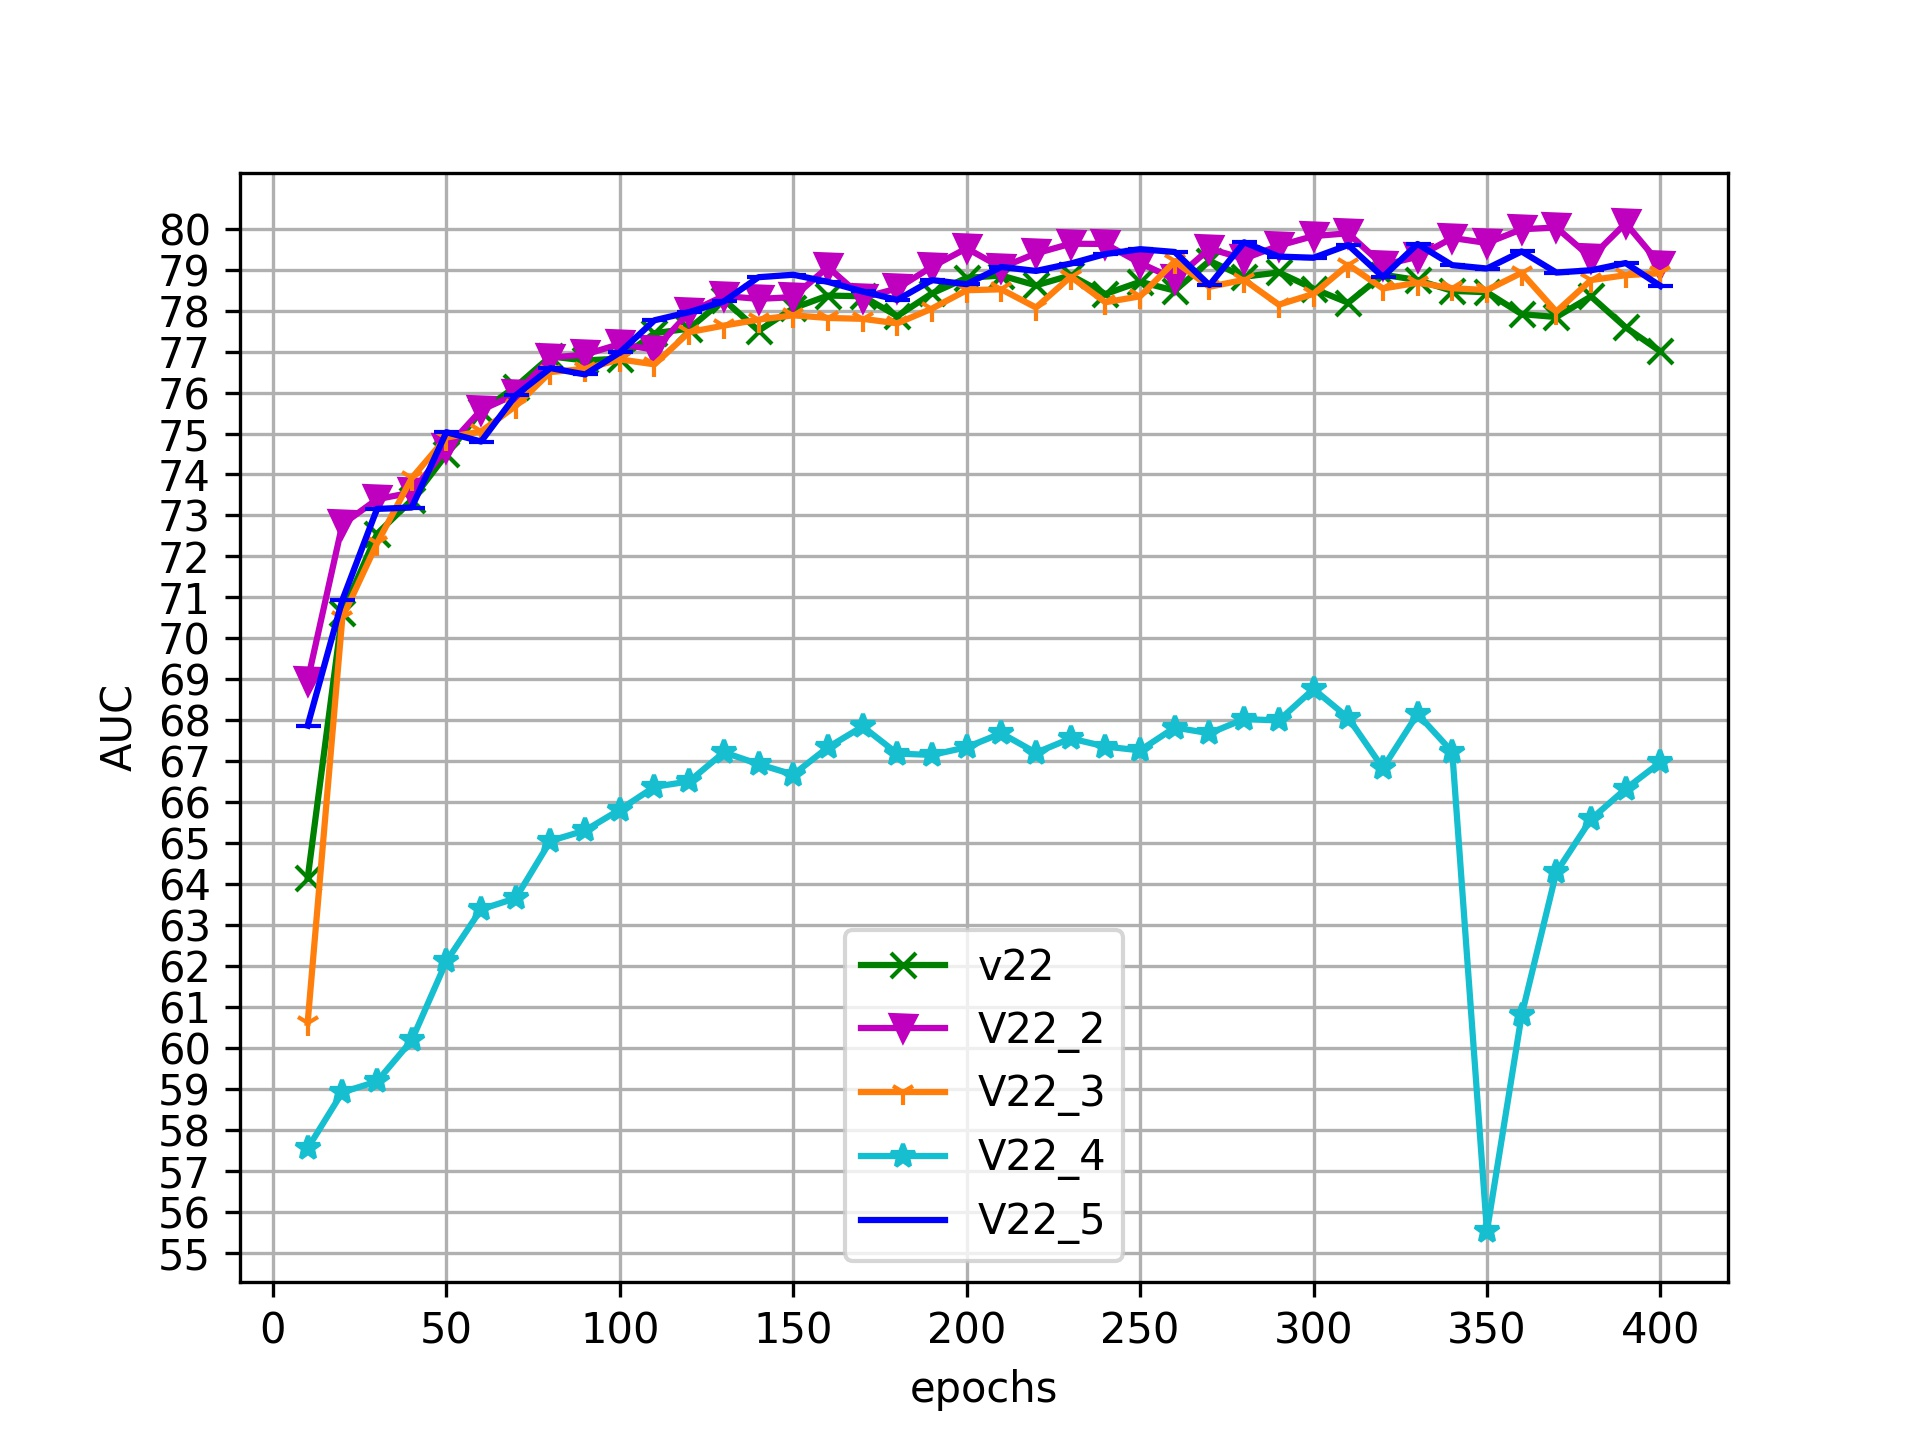
\includegraphics[trim=0 0 0 0, clip, width=1.\linewidth]{images/exp_1.jpg}
	\caption{Performance comparison changing the number of frames (from 1 to 5) in input of the Short-term memory module. NF: number of frames. \mnote{memento risolvere il crollo di NF1}}
	\label{fig:num-frames-vst}
\end{figure}

\begin{figure}[t]
\centering
	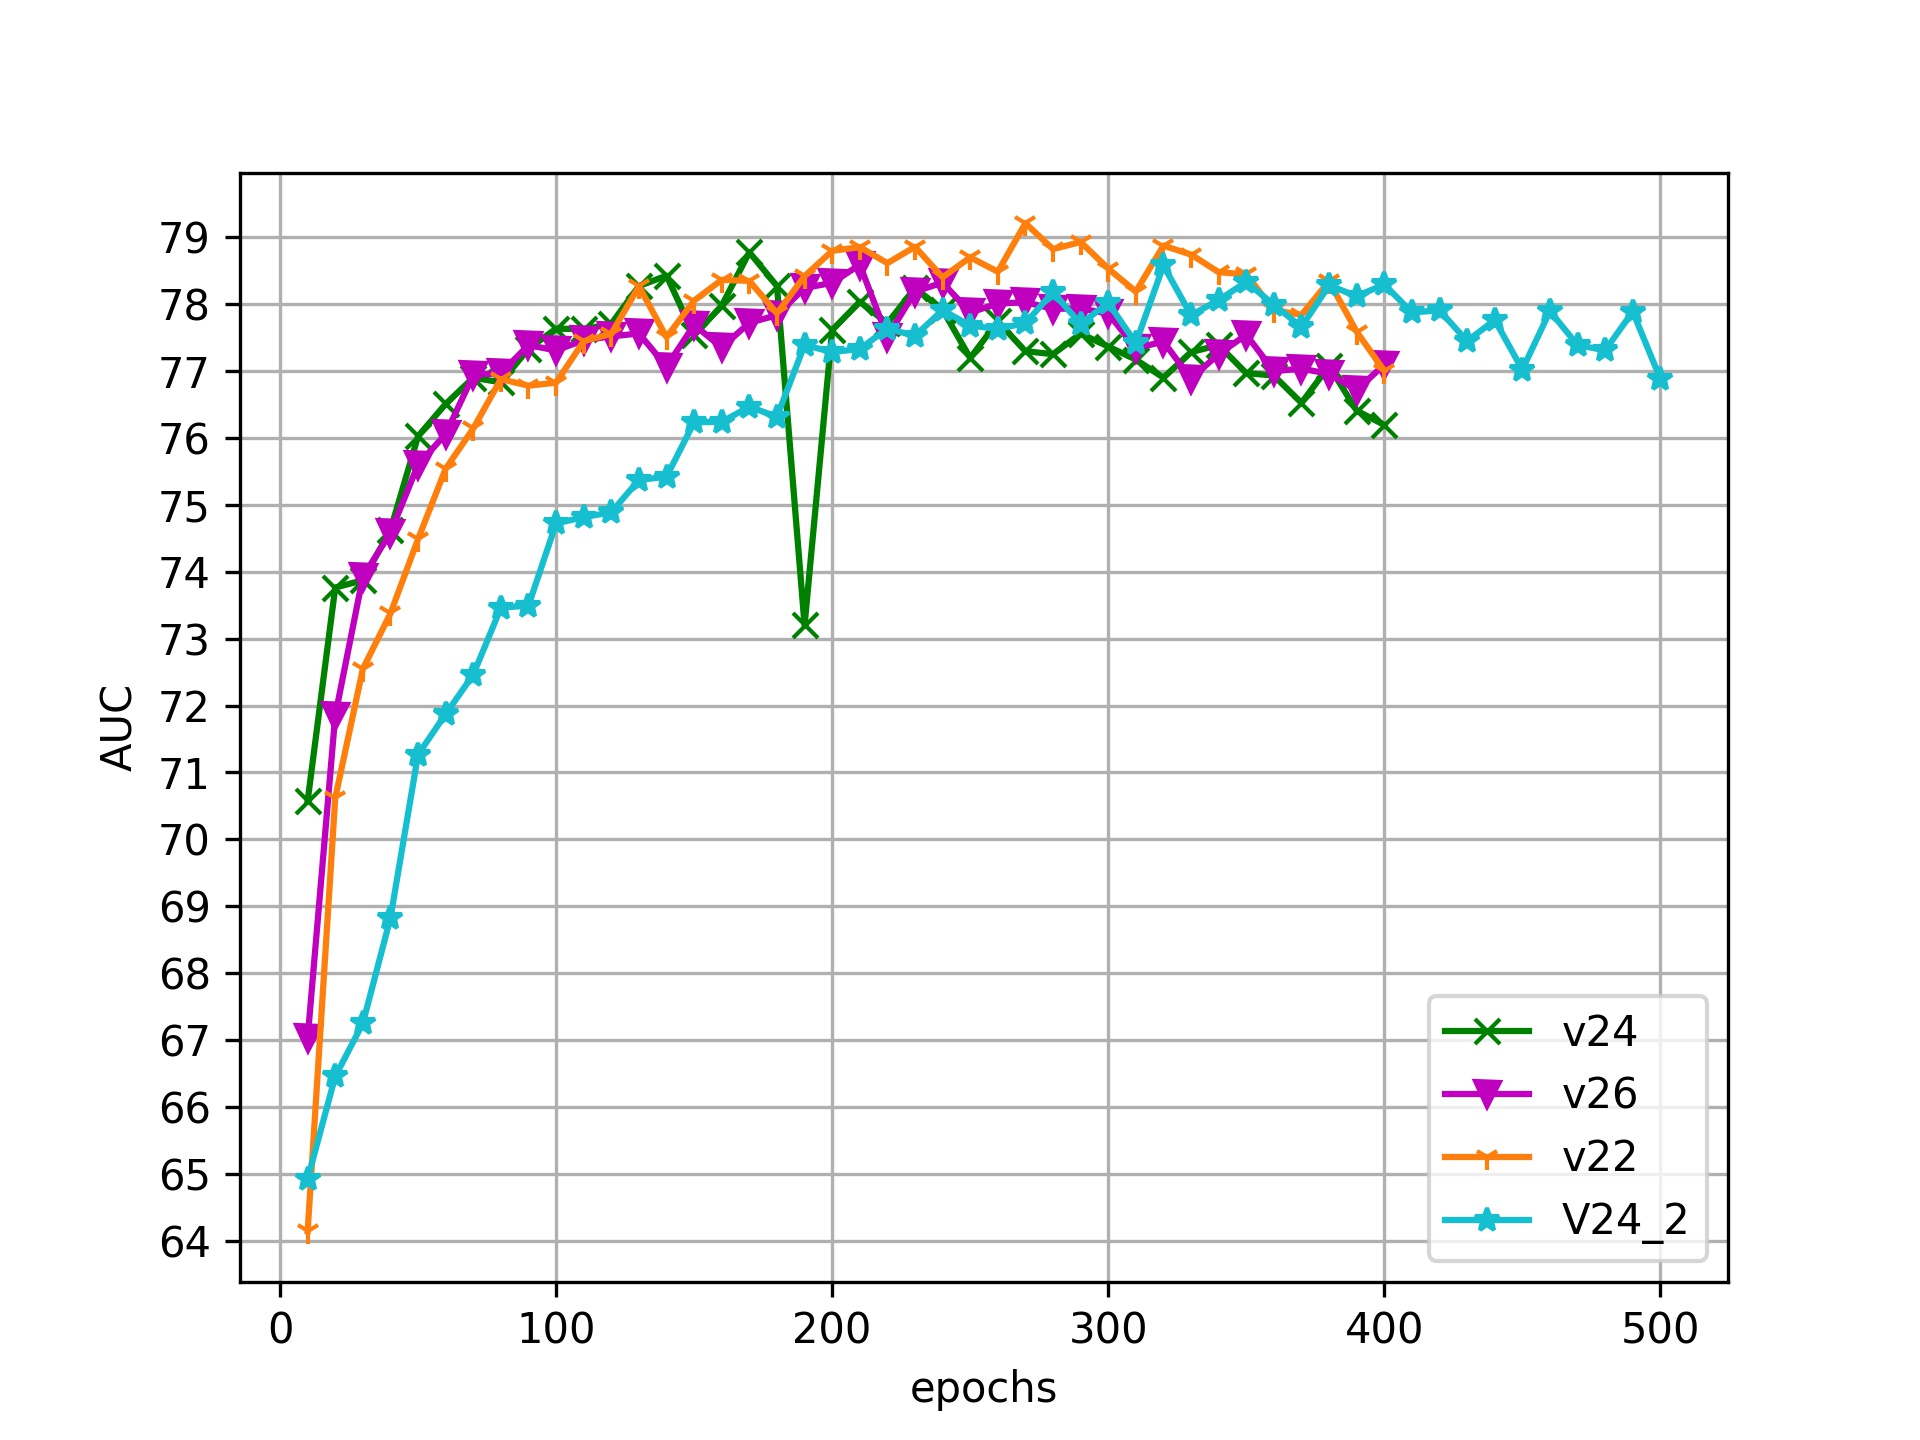
\includegraphics[trim=0 0 0 0, clip, width=1.\linewidth]{images/exp_2.jpg}
    % TODO aggiorna caption!
	\caption{Performance comparison changing the number of LSTM cells (from 0 to 4) that form the long-term memory. "LSTM 2 cells" is NF 3 of previous experiment in Fig.~\ref{fig:num-frames-vst}.}
	\label{fig:num-memory-cells}
\end{figure}

\begin{figure}[t]
\centering
	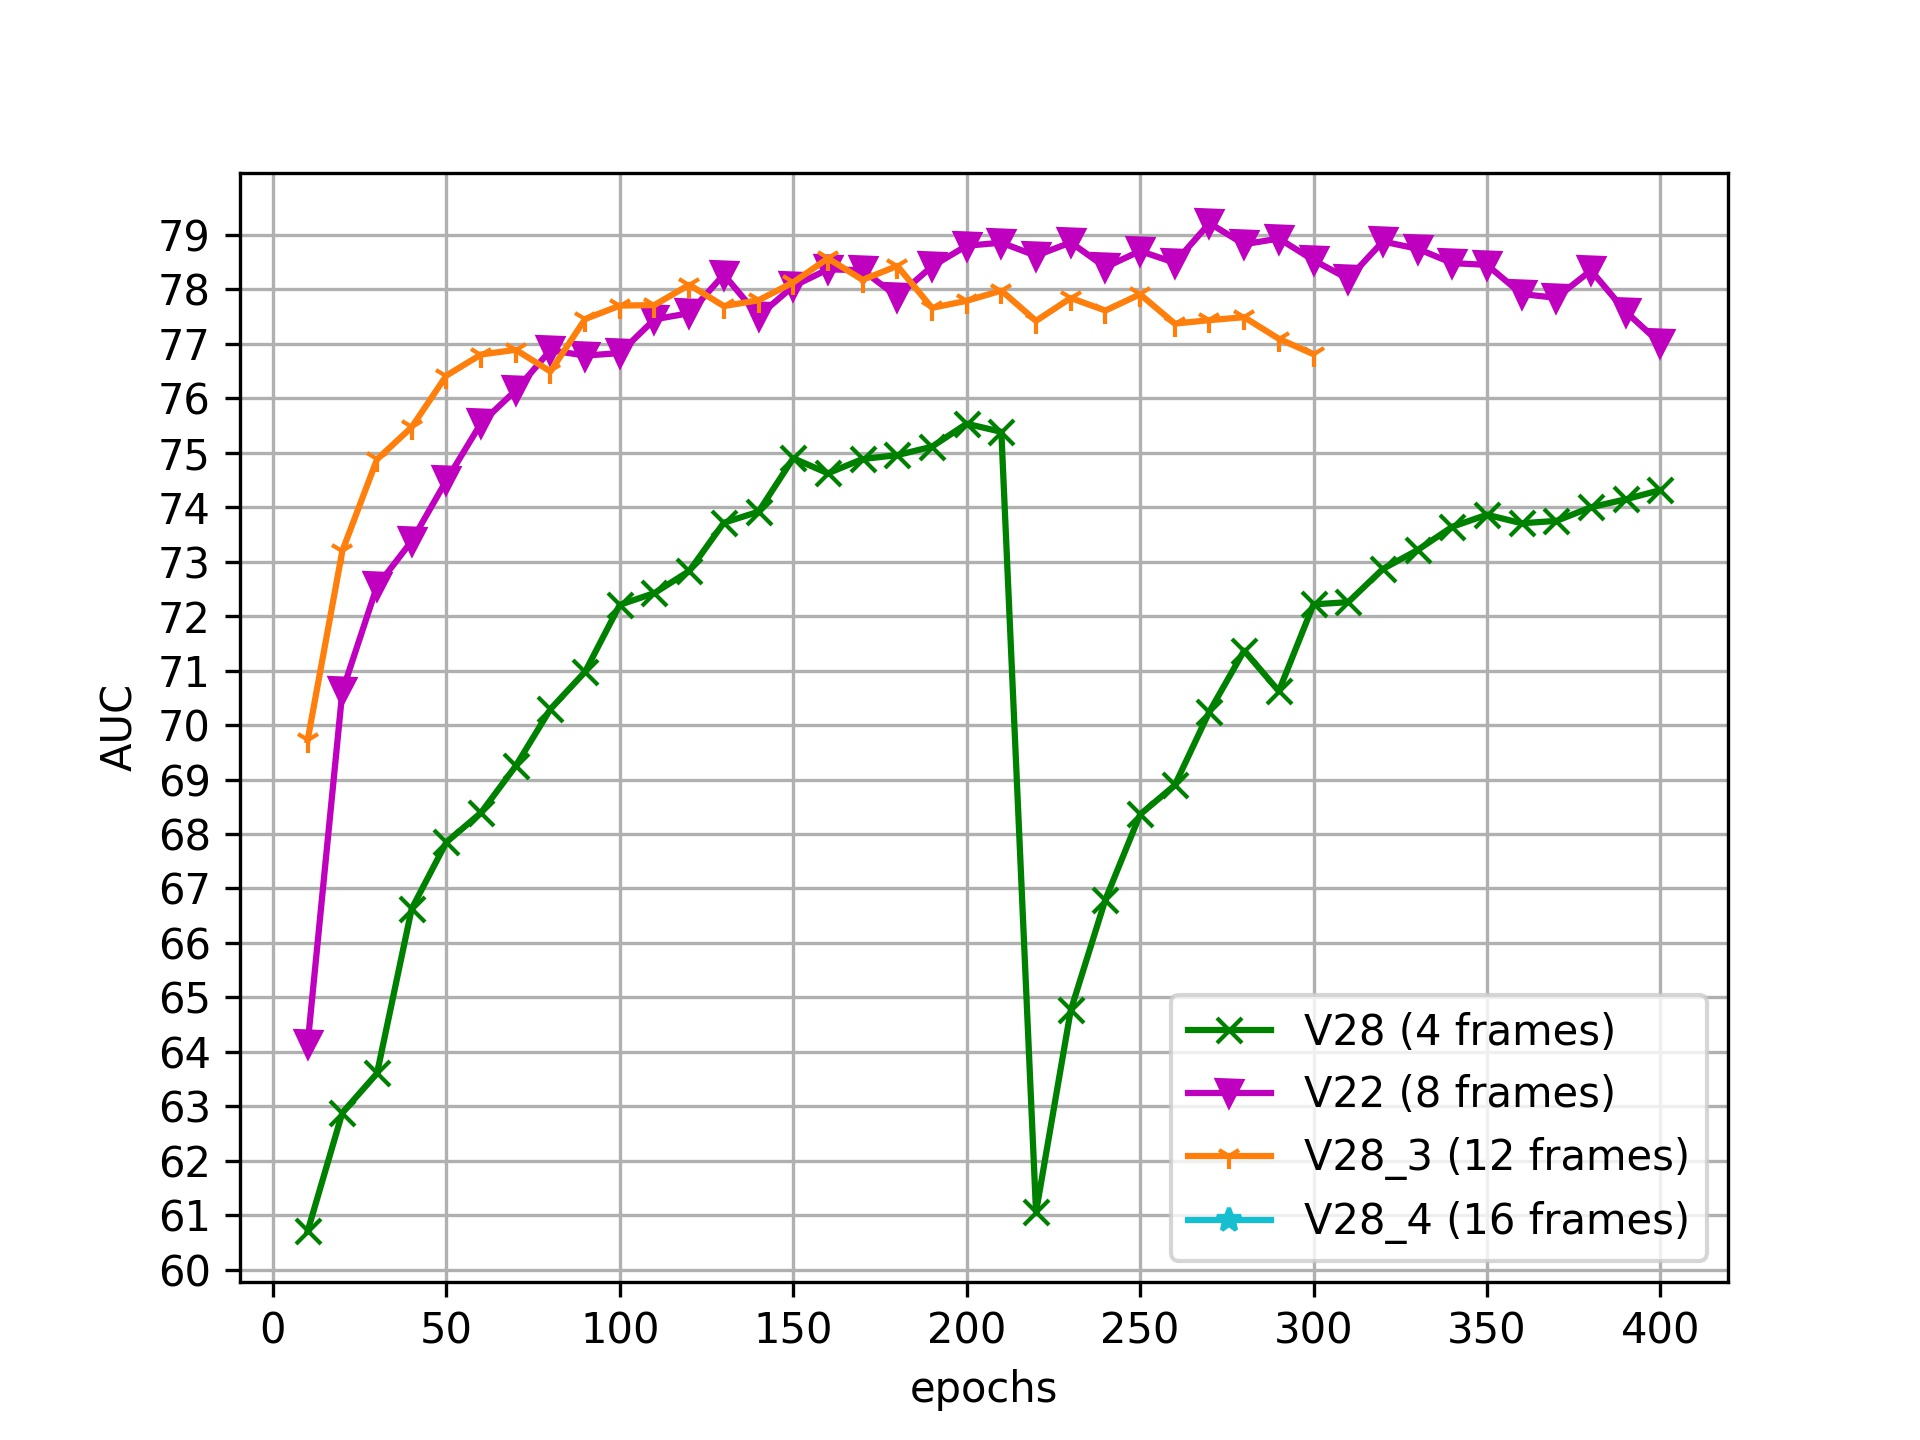
\includegraphics[trim=0 0 0 0, clip, width=1.\linewidth]{images/exp_3.jpg}
    % TODO aggiorna caption!
	\caption{Performance comparison changing the video clip length (from 4 to 16). The "8 frames" configuration is the NF 3 configuration of previous experiment in Fig.~\ref{fig:num-frames-vst}. \lnote{fix labels}}
	\label{fig:random-batch}
\end{figure}

\begin{table}[b]
	\footnotesize
	%\setlength{\tabcolsep}{1.2pt}
	\begin{center}
		\begin{tabular}{!r|^l|^l|^c|}
			\# & Method & Input & $AUC$ \\
			\hline\hline
	   	              1 & ConvAE \cite{hasan2016learning} & Gray & 64.3 \\
			        2 & ConvAE \cite{hasan2016learning} & Flow & 66.3 \\
                    3 & ConvLSTMAE \cite{chong2017abnormal} & Gray & 53.8 \\
                    4 & ConvLSTMAE \cite{chong2017abnormal} & Flow & 62.5 \\
                    5 & AnoPred \cite{liu2018future} & RGB & 67.5 \\
                    6 & AnoPred \cite{liu2018future} & Masked RGB & 64.8 \\
            \hline
                    7 & FOL-Ensemble \cite{9712446} & RGB + Box + Flow + Ego & 73.0 \\
                    8 & STFE \cite{zhou2022spatio} & RGB + Flow & 79.3 \\
            \hline
                    9 & Our (MOVAD) & RGB (320x240) &   \\
                    10 & Our (MOVAD) & RGB (640x480) &   \\
\end{tabular}
	\end{center}
	\caption{Benchmarks of VAD (Video Anomaly Detection) methods on the DoTA dataset.}
	\label{tab:sota-vad-auc}
\end{table}

% TODO visualizza anche la colonna OO e VO? (VO and OO columns are not shown because they do not contain anomalous traffic participants)
\begin{table*}[ht]
	\footnotesize
	\setlength{\tabcolsep}{5.0pt}
	\begin{center}
		\begin{tabular}{!l|^c|^c|^c|^c|^c|^c|^c|^c|^c|^c|^c|^c|^c|^c|}
			Model & $ST$ & $AH$ & $LA$ & $OC$ & $TC$ & $VP$ & $ST*$ & $AH*$ & $LA*$ & $OC*$ & $TC*$ & $VP*$ & $VO*$ & $OO*$ \\
			\hline\hline
                AnoPred \cite{liu2018future}        & 69.9 & 73.6 & 75.2 & 69.7 & 73.5 & 66.3 & 70.9 & 62.6 & 60.1 & 65.6 & 65.4 & 64.9 & 64.2 & 57.8 \\
                AnoPred \cite{liu2018future} + Mask & 66.3 & 72.2 & 64.2 & 65.4 & 65.6 & 66.6 & 72.9 & 63.7 & 60.6 & 66.9 & 65.7 & 64.0 & 58.8 & 59.9 \\
                FOL-STD \cite{9712446}              & 67.3 & 77.4 & 71.1 & 68.6 & 69.2 & 65.1 & 75.1 & 66.2 & 66.8 & 74.1 & 72.0 & 69.7 & 63.8 & 69.2 \\
                FOL-Ensemble \cite{9712446}         & 73.3 & 81.2 & 74.0 & 73.4 & 75.1 & 70.1 & 77.5 & 69.8 & 68.1 & 76.7 & 73.9 & 71.2 & 65.2 & 69.6 \\
                % STFE gli manca la colonna VP*!
                % STFE ha dei risultati non molto chiari.
                STFE \cite{zhou2022spatio} & 75.2 & 84.5 & 72.1 & 77.3 & 72.8 & 71.9 & 80.6 & 65.6 & 69.9 & 76.5 & 74.2 & N.D. & 75.6 & 70.5 \\
                Our (MOVAD) &      &      &      &      &       &      &      &      &      &      &      &      &    &   \\
                  % 
                  v30 & 84.2 & 85.8 & 83.6 & 82.3 & 84.9 & 83.2 & 73.7 & 71.6 & 73.0 & 80.6 & 78.0 & 73.9 & 80.2 & 77.6 \\
\end{tabular}
	\end{center}
	\caption{Detection accuracy for each individual accident category (AUC) on VAD task. "*" indicates non-ego anomaly categories. \lnote{mettiamo tutte le classi?}\vnote{secondo me si, sarebbe scorretto altrimenti, piuttosto evidenziamo le buone prestazioni in video ego}} 
	\label{tab:sota-vad-auc-per-class}
\end{table*}

\noindent\textbf{Dataset}.
We perform our tests on the DoTa dataset \cite{9712446}.
It contains 4677 videos taken from YouTube channels, with a resolution of $1280 \times 720$, annotated with information about the start and end of the anomaly, the category (10 in total) and the bounding boxes of the objects or persons involved.
The videos were recorded in different countries and with different light and weather conditions.
The dataset is split in approximately $70\%$ training and $30\%$ validation.
Our benchmarks are related to the Task~1~\cite{9712446}, the (frame-level) Video Anomaly Detection.
Our training and evaluation takes place in the most realistic, and most interesting condition from our point of view, online scenario.
That is, in which the model does not know what will happen in the future, but only know the present and the past.

\noindent\textbf{Evaluation Metrics}.
To evaluate the performance of the models, we use the well-known Area Under Curve (AUC) metric at frame-level.
This metric evaluate how well the model temporally locate the anomaly in the videos. 

\noindent\textbf{Implementation details.}
The results of the models with which we compare our model, are taken from the respective papers.
We perform the training on a single machine with 1 A100 GPU.
We use the Stochastic Gradient Descent (SGD) optimization algorithm with a learning rate of 0.0001, a momentum of 0.9, video clip length 8 and batch size 8.
We use SGD instead of Adam because in our experiments the latter led the training too much unstable, leading the model to diverge after a few epochs.

\noindent\textbf{Training details.}
Because the videos contain a non-uniform number of frames, to be able to fast training with batch-size major than one, we fixed the number of frames for each video taken into account, that is video clip length.
At each iteration we chose the starting frame for each video, adjusting the ground-truth accordingly, in a way to offer to the network as diverse as possible training and reduce the effect of overfitting.
Unless otherwise specified, the model is initialized using a uniform distribution for Linear weights, with a (semi) orthogonal matrix for LSTM modules and zero for bias parameters, the VST weights are initialized with a model pretrained on Something-Something v2 and input video shape is $320 \times 240$.

\subsection{Ablation study}

% class weight loss
% 2xsoftmax vs 1x
% learning rate differences (sto finendo l’esperimento con multipli lr)

\noindent\textbf{Short-term memory module.}

% v22: numero di frames in input
In this experiment, we empirically show the effects of the input frames to the Short-term memory module, varying the number of frames processed by the VST at each step.
The results are displayed in the Fig.~\ref{fig:num-frames-vst}.
As we expected, taking into account only the current frame is the worst situation, because most of the anomalies can be recognized by processing a wider time frame.
With 4 frames we have the best result.
Increasing the number of frames processed at each step has a much more limited effect.
While, already with 5 frames the effect become counterproductive.

% (no) v23: rand frame order (v17) vs normal
% v29_2, v29, v22: training from scratch vs pretrained (imagenet vs smth2smthv2)

\noindent\textbf{Long-term memory module.}
% posizione dell'lstm senza / prima / dopo / prim + dopo / gru
% v24_4: senza lstm
% v24, v22, v24_2: 1/2/3 # celle lstm
% v26, v26_2, v26_3: 1/2/3 # celle gru
% (no) v27, v27_2: pre + post lstm (1 cell) + saliency (?), pre + post lstm (1 cell)
In this experiment, we evaluate the long-term memory effect on the classification capability.
In Fig.~\ref{fig:num-memory-cells}, we compare the network with and without the LSTM long-term memory.
For the long-term memory, we test the LSTM and the GRU \cite{chung2014empirical} modules, with a number of cells varying from 1 to 4.
To make the Figure easier to read, the GRU results are not shown, but the trend does not differ much from the LSTM module. 
The effect introduced by the memory cells is evident.
Having no cell makes training slower in saturating performance and reach lowest AUC value.
With a cell, the performances saturate very quickly, with a slow degradation during the rest of the epochs.
By increasing the number of cells, the achievement of the maximum peak is slowed down over time, but in absolute value it is higher, converging towards similar values.
The maximum value is reached by 2 LSTM cells around epoch 270.
\lnote{check se aggiungere pezzo relativo a: alla fine la migliore è con 3 celle perchè il picco lo raggiunge verso 400 epoche quando interessa maggiormente a noi}

%\noindent\textbf{Saliency module.}
% v25, v22: con/senza/versione ridotta della saliency
%In this experiment, we evaluate the effect of the saliency branch.

\noindent\textbf{Video clip length.}
% v22, v28: random_batch 4/8/12/16/20/24: describi la modalità di addestramento -> per usare un batch size > 1 si è scelto di selezionare un numero max di frame da elaborare a ogni iterazione. per aggiungere diversità al training, il punto di inizio per ogni video viene scelto in modo casuale a ogni iterazione, adattando di conseguenza il ground-truth
As mentioned in training details subsection, at each iteration and separately for each video, a random starting point is selected and a fixed number of frames is inserted inside the batch to train the network.
In Figure \ref{fig:random-batch}, we evaluate the effect of the size of the video clip length.

\noindent\textbf{MOVAD model}
% input shape
% versione finale vs resto del mondo su dota, and: 
%   - Phantom: https://paperswithcode.com/paper/approaches-toward-physical-and-general-video
%   - ShanghaiTech: https://paperswithcode.com/sota/anomaly-detection-on-shanghaitech
%   - CUHK Avenue: https://paperswithcode.com/sota/anomaly-detection-on-chuk-avenue
%   - UCSD Ped2: https://paperswithcode.com/sota/abnormal-event-detection-in-video-on-ucsd
Finally, in Table \ref{tab:sota-vad-auc} we compare our architecture performance with state of the art models.
Table \ref{tab:sota-vad-auc-per-class} shows results per class.
\section{Conclusion}
\label{sec:conclusions}

In this paper, we proposed a new architecture called MOVAD for (online and frame-level) video anomaly detection.
Our model is composed by two modules: a short-term memory to extract information related to the ongoing action, implemented by a Video Swin Transformer adapted to work in a online scenario, and a long-term memory module that considers remote past information thanks to the use of a LSTM.
We evaluated the performance of our method on Detection of Traffic Anomaly (DoTA) dataset, a challenging collection of dash-mounted camera videos of accidents, and we reach an AUC score of \anote{82.05\%}, surpassing the current state-of-the-art by $+2.75\%$ AUC.

{\small
\bibliographystyle{ieee_fullname}
\bibliography{biblio}
}

\end{document}
